%%%%%%%%
\begin{figure}[!t]
\centering
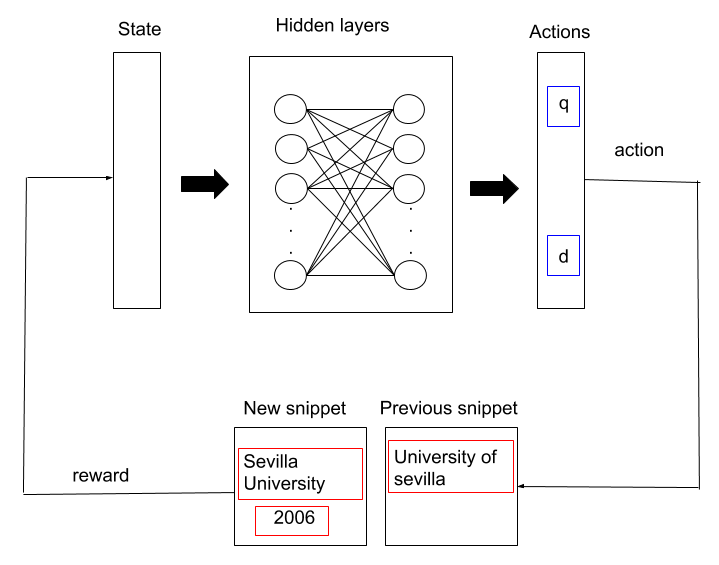
\includegraphics[scale=0.3]{./images/neural-network.png}
\caption{Deep Q-network framework for our web navigation system \PA{In Ivan's new experiments he proposed to replace the neural network with LSTM, while the input state is a new snippet.} \question{Since LSTM is for sequential learning approaches which part of our learning system is sequential?}}
\label{fig:naviagte}
\end{figure}
%%%%%%%%%

\paragraph{Queries: }  Since \textit{unoporuno} is an intelligent web navigation system, it requires some search engines and query generation models. In our work , we use four search engines including Google, DuckDuckGo, Researchgate, Citeceerx \PA{the search engine list should be modified. I didn't find the list.} . As person name is received from an available sociologist database, for each person we have $7$ possible number of queries as: \\

$<$person name$>$ $+$ (  $|$ doctorate $|$ institute $|$ master $|$ undergraduate $|$ university ) 

\paragraph{Markov Decision Process: } Using a similar framework as Narasimhan et al. \shortcite{narasimhan2016improving}, we model our web navigator model as a Markov Decision Process (MDP) \cite{puterman1994}. . .

This MDP is defined as a tuple $M(S, A, P, r, \gamma)$ where $S$ is a set of states, $A$ is a set of actions, $P :S\times A  \times S  \longrightarrow [0,1]$ is a transition function where $P(s'|s,a)$ encodes the probability of going to state $s'$ by being in state $s$, and choosing action $a$; $r : S \times A \longrightarrow R$ is a reward function (or penalty, if negative) obtained by choosing action $a$ in state $s$. Each parameter is detailed as the following.
\begin{itemize}
	\item The \textit{states} should be modeled in a way indicating the difference between the current and new snippets.  We use two models of sates in this paper (\question{I am wondering that there is no comparison between current and previous snippets in this model. I got the model from our code!}):
	\begin{itemize}
		\item \textit{Vector based}: each state indicates with a vector of real values containing: \\
		-- one-hot $7$ encoding indicating which query type is used for generating the snippet,\\
	    -- one-hot $4$ dimensional encoding indicating which research engine is used, \\
		-- number of common organisation names and dates between gold standards for a given person and extracted name entities in the new snippet,\\
        -- confident score for extracted organisation names and dates. 
		\item \textit{text based}: Each snippet is considered as a state ( \PA{for keeping this definition we should be certain about Ivan codes and results.} )
	\end{itemize}
	\item We have two \textit{Actions} including $q$ and $d$ indicating changing query and staying on the current query respectively. 
	\item The \textit{transition function} $P$ 
	\item The system goal is to extract the closest extracted organisation names and dates to the gold standards by generating less number of queries. For this reason, choosing $q$ action in any sate has a negative reward. And every time the extracted organisation name or date from a new snippet is close to the gold standards, the system receives a positive reward for instance $r(s, q) = -0.1$ or $r(s, d) = 10$ if the extracted organisation name (year) is in the list of organisation names (years) for the gold standards. 
\end{itemize}

%%%%%%%%%%%%%
\begin{algorithm}
 \KwData{Initialize an experience replay memory $\mathcal{D}$ with $N$ capacity (\PA{It should be explained in experiments})}
 Initialize a Q-value function $Q$ with random weight $\theta$\;
 \KwResult{$Q$-value function after training on snippets}
 \For{episode=0 \KwTo $M$ }{
 	get a random personid and initialise environment with start state $s_1$
 }
 \For{$t=1$ \KwTo $T$}{
	\eIf{random() $<\epsilon$}{ 
 	select a random action $a_t \in A$
 	}{$a_t = \text{argmax}_a Q(s_t, a; \theta)$}
 }
Execute action $a_t$ and obtain reward $r_t$ and new state $s_{t+1}$\\
$\mathcal{D} \longleftarrow (s_t, a_t, r_t, s_{t+1}) \cup \mathcal{D}$\\
sample eandom mini-batch of transitions $(s_j, a_j, r_j, s_{j+1}) $ from $\mathcal{D}$\\
\eIf{$s_{j+1}$ is terminal}{
	$y_j = r_j$
}{
	$y_j = r_j + \gamma \text{max}_{a'} Q(s_{j+1}, a';\theta)$ (\PA{this part should be explained and modified. Because we test double Q network too in the experiments.})
}
perform gradient descent on the loss $L(\theta)$ based on $y_j$ (\PA{that should be explained too})\\
\If{$s_{t+1}$ is a terminal state}{
\textbf{break}}
\BlankLine
 \caption{Training Procedure via Deep Q- Network (\question{may be it is not necessary to write its pseudo code again.})}
\end{algorithm}	
%%%%%%%%%%%%%